\documentclass[11pt,a4paper,polish,thesis]{dcsbook}

\usepackage[utf8]{inputenc}
\usepackage{babel}
\usepackage{graphicx} \graphicspath{ {images/} }
\usepackage[section]{placeins}
\setcounter{secnumdepth}{4}
\setcounter{tocdepth}{3}

\begin{document}
	
	\author{Tymoteusz Bleja \and Paweł Husak \and Patryk Imosa \and Magalena Łątkowska}
	\title{Internetowa gra edukacyjna ucząca podstaw pracy~z~programem~git}
	\subtitle{Praca inżynierska}
	\supervisor{dr~hab.~inż.~Marek Andrzej Wojciechowski}
	\date{Poznań, 2017}
	\maketitle
	\frontmatter
	\tableofcontents{}
	\mainmatter
	
	\chapter{Wstęp}
	
	\section{Zasady odnośnie pisania pracy}
	
	\begin{itemize}
	
		\item Piszemy w formie bezosobowej. Można też niby w 1.os liczby mnogiej czyli "Zrobiliśmy...", ale niektórzy akceptują tylko bezosobową, czyli "Zrobiono...".
		
		\item słów niepolskich - ,,Nie można więc bezpośrednio
		w tekście używać słów angielskich. Jeżeli już — powinny być wyróżnione kursywą'' - niektórzy podobno bardzo hejcą za angielskie słowa niestety.
			
		\item Jak chodzi o bibliografię, to w wolnej chwili dołączcie linki do stron z jakich korzystaliście, ja to potem ogarnę i zapiszę w takiej formie jak trzeba. Ale spokojnie, bo robienie bibliografii raczej zostawię na koniec.
		
		\item Ogólnie nie przejmujcie się strukturą, formatowaniem czy innymi formalnymi bzdetami, ja potem będę to ogarniać żeby było wg zasad więc nie traćcie czasu na ogarnianie takich rzeczy.
	\end{itemize}
	
	Między innymi: 
	skąd wgl pomysł - bo Git jest super i konieczny a ciężko się go samemu nauczyć, nauka z wielu źródeł jest chujowa, większość ma tylko blade pojęcie a potem idzie do pracy i dupa - co z tego że nauczyli się na studiach programować jak nie potrafią korzystać z Gita i współpracować z zespołem
		
	\section*{Cel i zakres pracy}
	
	cel - nauka fajna łatwa i przyjemna, oraz praktyczna, obycie z typowymi scenariuszami jakie mogą być potrzebne w pracy
	
	Coś o tym dlaczego akurat przeglądarkowa gra, czemu z grafiką 3D itp.
	
	Cytat z karty pracy : Zapoznanie się z systemem Git. Opracowanie koncepcji interaktywnego samouczka do nauki podstaw korzystania z systemu Git.  Opracowanie architektury systemu. Implementacja i testowanie systemu. Przygotowanie dokumentacji technicznej i użytkowej.
	
	\chapter{Podstawy teoretyczne}
	
	\section{Sysytem kontroli wersji Git}
	\textit{Może rozdział powinien się nazywać ,,Wstęp teoretyczny'', albo od razu ,,System kontroli wersji Git'' lub samo ,,Git'', i wtedy bez tej podsekcji - i tak w rozdziale nie może być tylko jedna}
	
	Krótki opis systemów kontroli wersji, do czego służą i jakie dają korzyści. Wyjaśnienie dlaczego Git się wyróżnia, co ma szczególnego i bardziej obszerny jego opis. 
	
	Jakaś subsekcja o tym dlaczego programiści powinny go znać i potrafić używać jako narzędzia w pracy, do czego im się przyda i że Git często nie jest możliwością, lecz koniecznością.
	
	\chapter{Projekt}
	
	\section{Założenia}
	
	Najważniejsze cele, co ma spełniać gra, czego ma nauczyć i w jaki sposób
	
	\section{Przebieg gry}
	
	Krótki opis rozgrywki i elementów interfejsu (może screeny? nie jestem pewna czy już w sekcji ,,projekt'' czy dopiero w sekcji ,,implementacja'')
	
	\section{Zadania}
	
	Ta sekcja nie tyle ma być o zadaniach w sensie Taskach, taskGraph.json itp, ale o zadaniach w kontekście co ma zrobić użytkownik, czego i w jaki sposób ma się przy tym nauczyć.
	
	Dzięki podziałowi zadania na kroki użytkownik uczy się jak należy postępować i jakich użyć komend, aby sprostać postawionemu zadaniu. Ma to również na celu automatyzowanie zachowania użytkownika w prawdziwych przypadkach, z którymi może się spotkać w domu lub pracy. Na każdy krok składa się opis co należy w nim zrealizować. W systemie git możliwe jest wykonanie pewnych akcji przy użyciu różnych komend czy przełączników.
	
	\subsection{Podpowiedzi/Pomoc}
	Nie wiem jak nazwać tę subsekcję, bo HelpDrawer to nie do końca pomoc czy podpowiedzi, tylko content do nauczenia, nie umiem tego ładnie nazwać na razie.
	
	Coś że gdy w zadaniu jest krok z nową komendą to wyskakuje pomoc i co w niej jest itp.
	
	\subsection{Punkty za rozwiązanie}
	%
	W projekcie wprowadzono elementy gamifikacji np. poprzez punkty za rozwiązanie zadań. Został dla nich stworzony komponent, który reaguje na zakończenie zadania. Przy wybieraniu zadania jako kolejne ustawiana jest wartość nagrody za poprawne wykonanie całego zadania. Wartość ta obliczana jest na podstawie minimalnego czasu przeznaczonego na dane zadanie pomnożonego przez ilość wykonanych zadań oraz liczbę 10. Co daje nam możliwość premiowania zadań, które są są wykonywane głębiej naszego drzewa zadań oraz mają być wykonane szybciej niż inne zdania. Gdy zadanie zostaje wykonane pobierany jest czas wykonania zadania. Jeżeli zadanie zostaje wykonane po przekroczeniu określonego na zadanie czasu użytkownik nie otrzymuje punktów. Natomiast jeżeli użytkownik zmieścił się w czasie, obliczona wcześniej nagroda zostaje pomnożona przez stosunek czasu, który został do czasu przeznaczonego na zadanie. Całość jest zaokrąglana w górę do liczby całkowitej. Obliczona wartość jest dodawana do całkowitej ilości punktów jaką dotychczas zdobył gracz. 

	% points with ranking ? ? ?

	Elementy takie jak punkty powodują, że gra wciąga użytkownika. Z każdym rozegraniem, użytkownik stara się pobić swój dotychczasowy wynik. W ten sposób co raz to szybciej i pewniej będzie wykonywał zadania oraz komendy. Dodatkowo punkty wprowadzają elementy rywalizacji pomiędzy użytkownikami. Użytkownicy będą starać się zajmować najwyższe miejsce w rankingu, co powoduję, że będą wykorzystywać aplikacje w celu uzyskania poprawy wyniku. 

	
	
	\chapter{Implementacja}
	
	\section{Wykorzystane technologie}
	
	\subsection{Redux}
	
	Wymagania dotyczące aplikacji przeglądarkowych stały się na tyle skomplikowane, że interfejs użytkownika jest bardzo złożony i może składać się z wielu elementów.
	Zarządzanie stanem takich aplikacji jest trudne, ponieważ występuje wiele zależności między komponentami. Może to doprowadzić do sytuacji, w której nie jest jasne co tak naprawdę się dzieje, a znalezienie błędów czy rozszerzenie funkcjonalności staje się zadaniem bardzo czasochłonnym i karkołomnym. 
	
	Jednym z rozwiązań jest właśnie skorzystanie z biblioteki Redux dla aplikacji pisanych w języku JavaScript. Głównym jej założeniem jest przejrzysty stan aplikacji, który może zmieniać się tylko w określonych momentach i~zawsze w~przewidywalny sposób. 
	
	Stan jest zdefiniowany jako zwykły obiekt o~strukturze drzewa, zawierający wszystkie możliwe informacje, jakie są potrzebne aby jednoznacznie określić i móc odtworzyć identyczną sytuację w aplikacji. Nie może on być modyfikowany, jest tylko do odczytu. Jedynym sposobem na jego zmianę jest wyemitowanie akcji, będącej po prostu zwykłym obiektem zawierającym obowiązkowo pole typ i dowolne inne potrzebne atrybuty.	Zadaniem akcji jest przejrzysty opis tego, co się wydarzyło w aplikacji, dzięki czemu dokładnie wiadomo co spowodowało zmianę. 
	
	Kluczowym elementem Reduxa są specyficzne funkcje, nazywane w języku angielskim \textit{reducers}, które definiują jak konkretna akcja wpływa na stan. Każda funkcja \textit{reducer} musi spełniać określone wymagania. Jako parametry przyjmuje zawsze tylko i wyłącznie obecny stan aplikacji i wyemitowaną akcję, a zwraca nowy obiekt stanu, w jakim znajduje się aplikacja na skutek wykonanej akcji. Ważne jest także aby \textit{reducer} był przewidywalny i deterministyczny. Oznacza to, że określony stan aplikacji i określona akcja spowodują powstanie zawsze takiego samego stanu. Dodatkowo taka funkcja nie może mieć żadnych skutków ubocznych. W dużych projektach wskazane jest napisanie kilku takich funkcji, z których każda modyfikuje tylko określoną część stanu. Ułatwia to utrzymanie zrozumiałego kodu, który można łatwo rozwijać i modyfikować.
	
	Podsumowując, Redux opiera się na trzech fundamentalnych zasadach:	
	\begin{itemize}
		\item cały stan aplikacji jest opisany przez pojedynczy obiekt o strukturze drzewa,
		\item jedynym sposobem aby zmienić stan aplikacji jest wyemitowanie akcji,
		\item wpływ danej akcji na sposób przekształcenia stanu określają funkcje zwane \textit{reducers}.
	\end{itemize}

	Popularność biblioteki Redux zasłużenie rośnie, ze~względu na~prostotę i~korzyści, jakie daje przestrzeganie opisanych wyżej trzech podstawowych reguł. Zdecydowano się skorzystać ~tej biblioteki ponieważ jest łatwa w~użyciu i pozwala w~wygodny sposób zarządzać stanem aplikacji. 
	
	\subsection{React.js}
	 
	 Jako bibliotekę do budowania interfejsu użytkownika wybrano bibliotekę React. 
	 Została ona stworzona w 2013 roku przez zespół programistów Facebook'a, aby rozwiązać problem tworzenia dużych aplikacji, w których nieustannie zmienia się to, co należy wyświetlać. Początkowo nie była ona ogólnodostępna, ale aktualnie jest udostępniona na zasadzie otwartego źródła (ang. \textit{open-source}) w serwisie github.com. React pozwala określić jak aplikacja powinna wyglądać w różnych momentach, a samo odświeżanie interfejsu dzieje się automatycznie, gdy zmienią się dane dotyczące komponentów. Dodatkowo ogromną zaletą tej biblioteki jest fakt, że potrafi ona określić co dokładnie uległo zmianie, a~w~rezultacie ponownie wyrenderowć tylko fragmenty, które rzeczywiście tego wymagają.
	 
	 React opiera się na koncepcji niezależnych komponentów, nadających się do~wielokrotnego wykorzystania, z~których można komponować skomplikowane widoki. Są to obiekty JavaScript, reprezentujące elementy HTML, czyli w~istocie fragmenty interfejsu użytkownika, mające określoną strukturę i~funkcjonalność.
	 
	 Wykorzystywany jest też wirtualny obiektowy model elementu (ang. \textit{virtual DOM}), czyli obiekt o strukturze drzewa, zbudowany z wcześniej zdefiniowanych komponentów. React obserwuje, czy nie nastąpiły żadne zmiany w~nim, a~jeżeli tak, to automatycznie modyfikuje rzeczywisty i~widoczny dla użytkownika DOM, tak aby odzwierciedlał on stan wirtualnego DOM. Istotne jest, że~odświeżeniu podlegają tylko te fragmenty, które uległy zmianie.
	 
	 Kluczową rolę pełni funkcja \textit{render}, przyjmująca dwa parametry --- wirtualny element oraz węzeł DOM, w którym umieszczony zostanie dany element. Dopiero jej wywołanie powoduje, że komponent jest widoczny w przeglądarce. Każdy z takich elementów może mieć właściwości (ang.\textit{props}) oraz przechowywać swój własny wewnętrzny stan (ang. \textit{state}). Różnica między nimi jest taka, że właściwości powinny być stałe, a stan może się zmieniać w czasie. Jego zmiana wywołuje metodę \textit{render()}, odświeżającą komponent.
	
	Zdecydowano się na wykorzystanie biblioteki React.js, ponieważ aplikacje napisane z~jej użyciem wymagają mniejszego nakładu pracy aby działać responsywnie i szybko. Dodatkowo biblioteka ta doskonale współpracuje z Reduxem, w którym stan całej aplikacji przechowywany jest w jednym obiekcie nazywanym stanem. Wystarczy odpowiednie jego fragmenty podpiąć do konkretnych komponentów, aby interfejs automatycznie reagował na jego zmiany. 
		
		
	\subsection{Babylon.js}

	Babylon.js jest otwartą biblioteką WebGL napisaną w TypeScript wykorzystywaną przede wszystkim do tworzenia gier wideo w przeglądarkach. Pierwsza odsłona została wydana w 2013 roku. Głównymi twórcami są David Cotuhe oraz David Rousset. Jako, że jest silnikiem 3D posiada wspaniałe narzędzia do tworzenia, wyświetlania i teksturowania szkieletów w przestrzeni. Przez to, że kierowana jest głównie do twórców gier posiada wiele dodatkowych funkcji jak generowanie krawędzi, gotowych obiektów ułatwiających pracę programiście typu tworzenia obiektu na podstawie mapy wysokości. Ponadto zapewnia natywną detekcję kolizji, grawitację sceny, czy wbudowane kamery np. FollowCamera - kamera śledząca, automatycznie podążająca za obiektem. 
	
	Rozważana była jeszcze inna biblioteka 3D, a mianowicie Three.js wydana w 2009 roku, również oparta na podstawie webGL. Po zapoznaniu i przetestowaniu obu silników wybór padł na Babylon.js. Głównymi czynnikami skłaniającymi nas w stronę Babylon'a była płynność, którą zapewniał w przeciwieństwie do Three.js oraz prostota użycia. Przy renderowaniu tego samego, wybranego obiektu Babylon.js spisywał się lepiej o kilka klatek. Poza tym Babylon.js jest dobrze udokumentowany, posiada bogatą bazę poradników oraz społeczność wykorzystujące tę bibliotekę jest duża i stale rośnie.
	
	\subsection{Pozostałe?}
	
	\section{Scenariusz rozgrywki}
	
	\subsection{Struktura} \label{Struktura}
	
	Scenariusz rozgrywki to skierowany graf, którego wierzchołkami są zadania, z~których każde składa się z~kilku kroków. Zdecydowano się na taką strukturę ze względu na to, że daje ona możliwość sekwencjonowania zadań, a zarazem pozwala na element losowości. Jeżeli z wierzchołka dotyczącego jakiegoś zadania wychodzi kilka krawędzi, to kolejny węzeł, czyli kolejne zadanie, wybierane jest w sposób losowy spośród sąsiadów aktualnego wierzchołka. Dzięki takiej reprezentacji nigdy nie zdarzy się sytuacja, w której następnym zadaniem będzie zadanie nieadekwatne do aktualnego stanu repozytorium.

	\subsubsection{Konstrukcja zadania}
	Pojedyncze zadanie reprezentowane jest w postaci obiektu, który składa się z następujących pól:
	\begin{itemize}
	\item identyfikator,
	\item zbiór identyfikatorów możliwych następników,
	\item tytuł,
	\item opis,
	\item minimalny czas,
	\item domyślny (maksymalny) czas,
	\item lista kroków.	
	\end{itemize}
	
	Opis zadania służy ukazaniu użytkownikowi celu oraz problemu, jaki należy rozwiązać w danym zadaniu. Może to być na przykład rozszerzenie funkcjonalności lub naprawa błędu.
	
	\textit{Aby nagradzać użytkownika punktami za szybko wykonane zadanie, zdecydowano się na określenie czasu na wykonanie zadania. Jest on obliczany w momencie dodawania nowego zadania na podstawie ilości dotychczas wykonanych zadań, a także wartości minimalnej oraz maksymalnej czasu zdefiniowanych w danym zadaniu.}
	
	Zbiór następników zawiera identyfikatory zadań, które mogą wystąpić po aktualnym. Hierarchia zadań ułożona jest w postaci grafu skierowanego, tak więc wszystkie wierzchołki, do których istnieją krawędzie wychodzące z wierzchołka reprezentującego dane zadanie, są jego następnikami. 
	
	Kluczowym elementem zadania jest uporządkowana lista kroków, które należy wykonać, aby rozwiązać zadanie i przejść do kolejnego. Wykonanie kroku polega na wpisaniu odpowiedniej komendy systemu Git. Szczegółowy opis jego konstrukcji w kolejnej sekcji.

	
	\subsubsection{Konstrukcja kroku}
	
	Podobnie jak zadanie, krok jest obiektem składającym się z kilku pól, a mianowicie:
	\begin{itemize}
		\item typ,
		\item opis,
		\item lista dozwolonych poleceń,
		\item etykiety,
		\item dodatkowe dane, charakterystyczne dla danego typu kroku.	
	\end{itemize}

	Typ określa jakiej komendy systemu Git dany krok dotyczy. Obsługiwane typy to m.in. ''COMMIT'' czy ''MERGE''. Na podstawie typu poprawnie wykonanego kroku określana jest akcja, jaką należy wykonać po stronie grafiki 3D, by odwzorować aktualny stan repozytorium. 
	 
	W opisie znajduje się krótka informacja, co należy zrobić, aby wykonać krok i przejść do kolejnego. Krok jest uznawany za wykonany, gdy użytkownik wpisze w konsoli jedno z~poleceń z~listy dozwolonych komend i~zatwierdzi je.
	
	Do każdego kroku przypisana jest lista etykiet, określających jakiego zagadnienia dotyczy dany krok. Krok posiada zawsze co najmniej jedną etykietę, wskazującą komendę, której wymaga on do poprawnego wykonania. Gdy użytkownik poprawnie zrealizuje dany krok, to zwiększany jest wskaźnik powodzenia dla wszystkich przypisanych do niego etykiet. Poza wspomnianym wskaźnikiem przechowywana jest także ilość poprawnych wywołań komendy. Informacje te umożliwiają określenie stopnia, w jakim użytkownik opanował dane zagadnienie i nad czym powinien jeszcze popracować. Brane jest to pod uwagę przy losowaniu kolejnych zadań. Dla możliwych następników wyliczana jest waga na podstawie etykiet, jakie mają w swoich krokach. 
	
	\textit{Obliczenie wagi dla zadania polega na zsumowaniu kwadratów ilorazu wartości 1 oraz wyznaczonego wskaźnika dla kolejnych etykiet w krokach zadania, będącego ilorazem poprawnie wykonanych kroków z całkowitą liczbą prób dla tej etykiety. Dzięki takiemu zabiegowi zwiększane jest prawdopodobieństwo wylosowania kolejnego zadania poruszającego zagadnienia, z~którymi użytkownik nie radził sobie zbyt dobrze.}
	
	Dodatkowe dane, w zależności od typu kroku, mogą składać się z różnych elementów. Dostarczają informację np. o nazwie wykonanej rewizji czy utworzonej gałęzi. Służą też do określenia jakie pliki powinny zostać dodane lub usunięte z repozytorium. W przypadku kroku dotyczącego polecenia \textit{git checkout} przechowują informację, czy przełączenie powinno być zrealizowane na konkretną gałąź czy rewizję.
	
	\subsubsection{Format danych}
	
	Jak opisano wcześniej, scenariusz rozgrywki to w istocie struktura drzewiasta złożona z zadań, przy czym każde z nich zawiera pewne informacje oraz uporządkowaną listę kroków. Tak złożony obiekt wymagał odpowiedniego i wygodnego formatu do przechowywania danych. Zdecydowano się na format JSON, który doskonale nadaje się do tego celu. Pliki zapisane w tym formacie można bezproblemowo odczytywać oraz modyfikować za pomocą języka JavaScript.
	
	\subsection{Graficzne narzędzie do definiowania scenariuszy}
	
	\subsubsection{Motywacja}
	
	Aplikacja GITar Hero umożliwia przetwarzanie rozbudowanych scenariuszy, których ręczne tworzenie byłoby uciążliwe i  czasochłonne, a ponadto podatne na błędy. Dodawanie lub modyfikacja zadań wymagałaby znaczących nakładów pracy.
	Z tego względu zdecydowano się na korzystanie z narzędzia z graficznym interfejsem użytkownika, za pomocą którego można by było w prosty i wygodny sposób tworzyć grafy zadań oraz zapisywać je w formacie JSON. 
	
	\subsubsection{Poszukiwanie gotowego rozwiązania}
	
	Początkowo zamierzano skorzystać z gotowego rozwiązania. Do tego zadania wytypowano aplikację \textit{directed-graph-creator} użytkownika cjrd [tu odnosnik do bibliografii i tam link] udostępnianą jako oprogramowanie o~otwartym źródle (ang. \textit{open source}) \footnote{Oprogramowanie udostępnione jest na licencji MIT/X, dzięki czemu istnieje nieograniczone prawo do używania, kopiowania, modyfikowania i~rozpowszechniania go. Jedynym wymogiem jest, by we wszystkich wersjach zachowano warunki licencyjne oraz informacje o autorze.}. Umożliwia ona tworzenie grafów skierowanych oraz~ich zapis do formatu JSON. Narzędzie to jest zaimplementowane w języku JavaScript i~korzysta z popularnej biblioteki~D3.js, która pozwala tworzyć dynamiczne i~interaktywne wizualizacje danych w~przeglądarkach internetowych.
	
	Jednakże aplikacja, w~formie w jakiej została udostępniona, nie wystarczała do zdefiniowania scenariusza rozgrywki. Każdy węzeł grafu mógł przechowywać tylko pojedynczy ciąg znaków. Potrzebne były zatem znaczne modyfikacje, umożliwiające zapisanie w pojedynczym węźle wszystkich niezbędnych informacji, które powinny się znaleźć w zadaniu. Zdecydowano się zatem stworzyć własne narzędzie do~tworzenia scenariusza zadań, bazujące na ogólnodostępnym \textit{direct-graph-creator}.
	
	\subsubsection{TaskCreator}
	
	Postanowiono przerobić wspomnianą wyżej aplikację. Została ona napisana tylko i wyłącznie w języku JavaScript, bez wykorzystania jakichkolwiek platform programistycznych (ang. \textit{frameworks}). Modyfikację utrudniał także fakt, że cały kod zawarty był w~jednym pliku. Postanowiono nie modyfikować struktury aplikacji i~dalszą część napisać również w czystym języku JavaScript. Dodano jedynie bibliotekę jQuery, która umożliwia łatwiejsze zarządzanie elementami drzewa DOM, czyli obiektowego modelu dokumentu. W~związku z~tym, że jest to aplikacja internetowa, potrzebny był serwer HTTP. W~tym celu użyto środowiska Node.js, wykorzystywanego do tworzenia wysoce skalowalnych aplikacji sieciowych.
		
	\begin{figure}
		\centering
		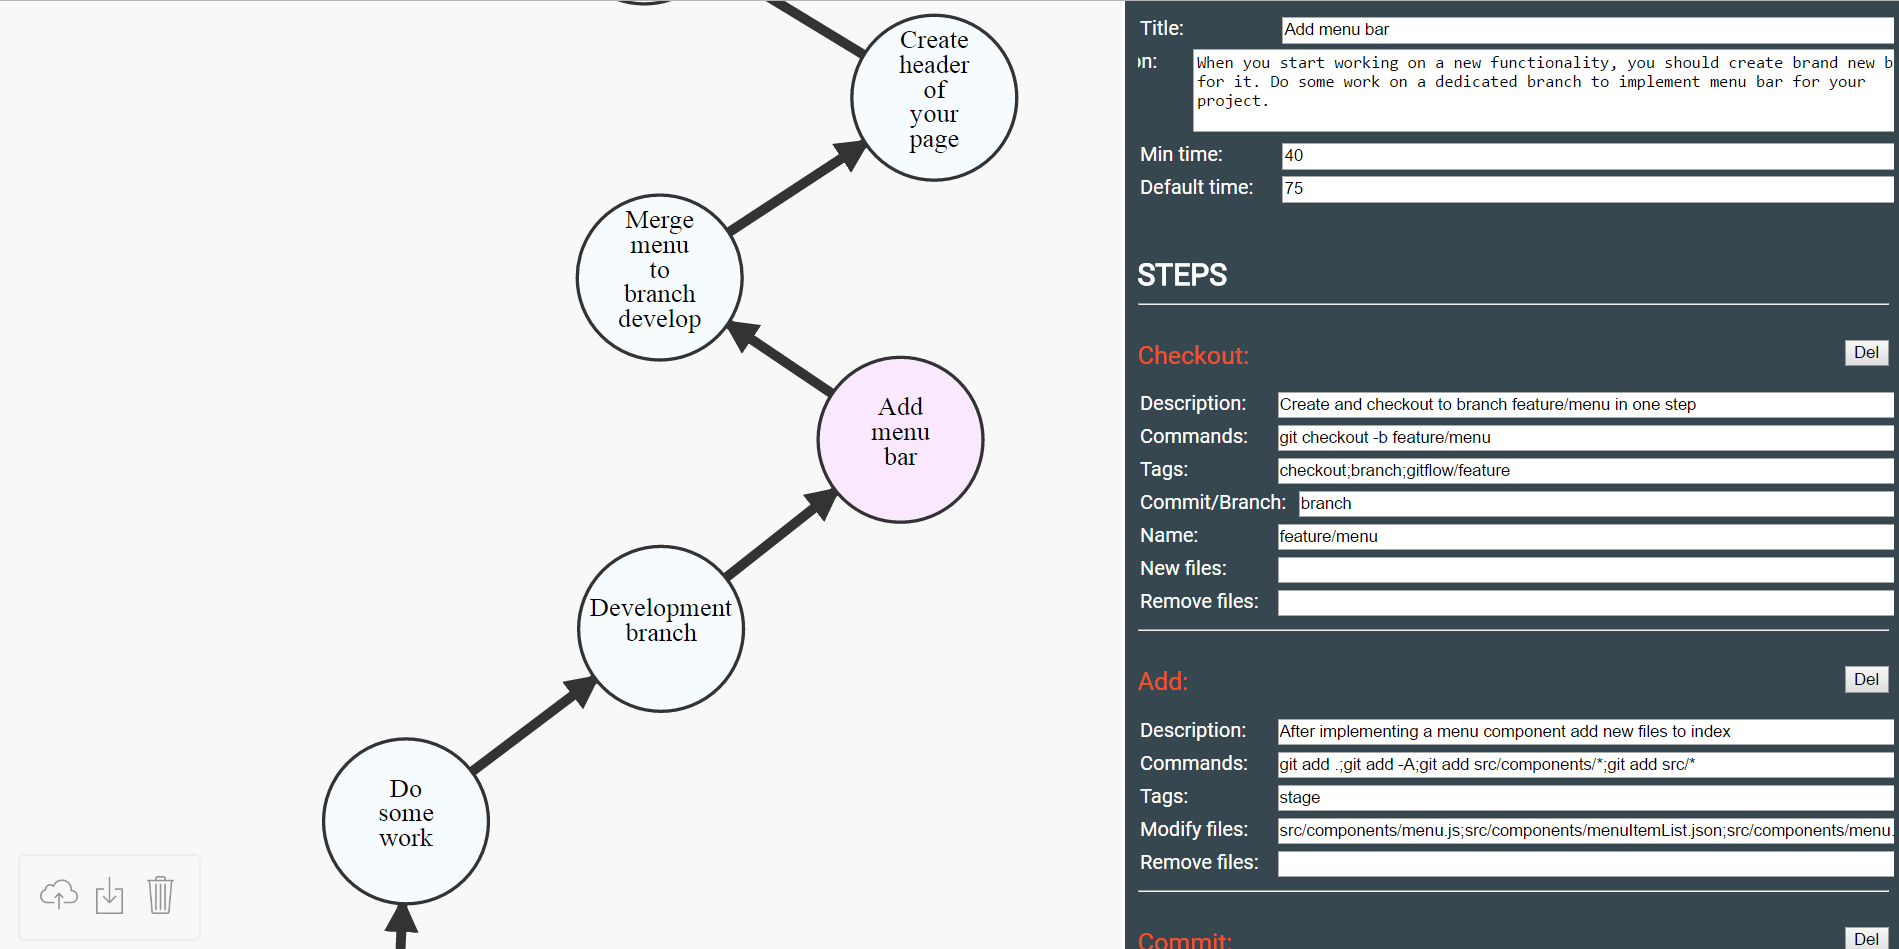
\includegraphics[width=15cm]{graphCreator01}
		\caption{Interfejs graficzny graphCreatora}
		\label{fig:graphCreator}
	\end{figure}
	
	Największą modyfikacją było rozszerzenie interfejsu o dodatkowy panel boczny służący do wypełniania pól zadania i definiowania listy kroków. Jest on widoczny na rysunku~\ref{fig:graphCreator} po prawej stronie. Po~kliknięciu na węzeł grafu, reprezentujący pojedyncze zadanie, na bocznym panelu zostają wyświetlone wszystkie informacje dotyczącego wybranego elementu. Należą do nich między innymi tytuł, opis oraz czasy wykonania. Oczywiście wszystkie pola są edytowalne. W panelu istnieje również możliwość definiowania listy kroków, które trzeba zrealizować żeby wykonać zadanie. Aby dodać jeden z nich należy wybrać jego typ i kliknąć przycisk "Dodaj", a następnie wypełnić pola opisujące dany krok. Znajdują się tam atrybuty takie jak opis, lista komend spełniająca dany krok, etykiety opisujące wykonane czynności jak również dodatkowe parametry, charakterystyczne dla poszczególnych typów kroków. 
	
	Aby dodać nowy węzeł grafu należy przytrzymać klawisz Shift i kliknąć myszką w wybrane miejsce. Żeby edytować wierzchołek należy go wybrać poprzez kliknięcie. Z kolei przytrzymanie klawisza Shift oraz wciśniętego lewego przycisku myszki a następnie przeciągniecie kursora znad jednego węzła na drugi utworzy skierowaną krawędź między nimi. Aby usunąć wybrany wierzchołek grafu bądź jego krawędź, należy go zaznaczyć kliknięciem oraz nacisnąć klawisz Delete. 
	
	Stworzony w ten sposób graf zadań można zapisać do formatu JSON. W tym celu wystarczy kliknąć drugi przycisk w lewym dolnym rogu ekranu. Narzędzie wygeneruje strukturę grafu zrozumiałą dla aplikacji GITar Hero, określi zadanie inicjujące rozgrywkę i zapisze dane do pliku taskGraph.json. Zapisane w ten sposób grafy można wczytać ponownie do aplikacji graphCreator naciskając pierwszy przycisk w lewym dolnym rogu ekranu i wybierając plik do wczytania.
	
	\section{Komponenty/elementy(?) aplikacji}
	
	\subsection{Lista zadań}
	
	Screen jakiś, jak działa, o implementacji
	
	\subsection{Konsola}
	
	Screen jakiś, jak działa, o implementacji
	
	\subsection{Pomoc (HelpDrawer)}
	
	Screen jakiś, jak działa, o implementacji
	
	\subsection{Drzewko repo}
	
	Screen jakiś, jak działa, o implementacji
	
	\subsection{Canvas}
	
	W projekcie skorzystano z komponentu 'canvas' z html w wersji 5. Pozwala on na wyświetlanie grafiki w przeglądarce. Służy jako kontener dla graficznego silnika 3D, pochodzącego z biblioteki babylon. 
	
	\section{Grafika 3D}
	Tu będzie sporo, do tego stopnie sporo, że nie wiem jeszcze jak to zaplanować i porozdzielać, względem czego.
	
	Czy np podsekcje takie jak:
	repo3d - gałęzie, commity, co to są i jak powstają na akcje, o ich teksturze, obramowaniu, w tym o solidExplode
	ground - co to, jak działa itp
	particle w tle
	(wg elementów aplikacji)
	
	Czy może raczej podsekcje wg 'elementów' Babylona:
	Meshe, SolidParticle, Particle, Materiały, Tekstury, Shadery
	
	

	\subsection{Repozytorium 3D}
		Aby odwzorowywać stan repozytorium na ekranie został stworzony odpowiedni kontroler. Ma on za zadanie reagować na realizowane przez użytkownika komendy i zarządzać elementami grafiki 3D. Nasłuchuje na wykonywane akcje i w zależności od ich typu dodaje, usuwa bądź modyfikuje elementy na scenie. W kontroler ten zawiera listę gałęzi będących w stanie repozytorium. % husaku i imosiaku

	\subsection{Branch}
	Obiekt 3D reprezentujący gałąź systemu git jest tworzony przy pomocy funkcji CreateTube z biblioteki Babylon.js. 
	Funkcja ta generuje siatkę wierzchołków, na podstawie podanej listy punktów określających ścieżkę, w kształcie tuby. Pozwala również na określenie średnicy oraz
	szczegółowości siatki. Parametry te zostały dobrane w taki sposób, aby wygenerować tubę, której przekrój przypomina koło przy jednoczesnym zachowaniu jak najmniejszej liczby użytych wierzchołków. Jedna gałąź może składać się z dwóch rodzajów siatki. Pierwsza z nich reprezentuje główny człon. Ścieżka użyta do jej wygenerowania zawiera tylko dwa punkty wyznaczające początek i koniec tuby. Dzięki temu można osiągnąć dowolnie długi odcinek nie zwiększając przy tym liczby wierzchołków. SPRAWDZIC I OPISAC PROBLEM Z IN FRUSTRUM. Drugi rodzaj siatki wykorzystywany jest do wygenerowania tuby będącej łącznikiem między gąłęziami. Do wyznaczenia ścieżki skorzystano z funkcji pomocniczej generującą krzywą Beziera. Funkcja ta przyjmuje dwa punkty określające początek i koniec ścieżki oraz dwa inne określające jej kształt. SPRAWDZIC KRZYWE BEZIERA. 
	% husaku i imosiaku

	\subsection{Commit}
	Zatwierdzenie zmian w repozytorium git w grafice trójwymiarowej jest przedstawione w postaci kuli umieszczonej na gałęzi, której dotyczy. Funkcja CreateSphere pochodząca z babylon'a buduje siatkę wierzchołków w kształcie sfery o określonej średnicy oraz teselacji. Przy wartości teselacji równej szesnaście powierzchnia obiektu wygląda na wygładzoną. W momencie utworzenia kuli  pojawia się nad nią napis z wiadomością przekazywaną przy zatwierdzaniu zmian, którego kolor jest niewiele jaśniejszy niż kolor samego obiektu. Ponadto może również zostać dodany tekst z numerem wersji tzw. tag, znajdujący się nieco powyżej tekstu z wiadomością. Sam tekst jest wyświetlany tylko dla 'commitów' na gałęzi, na której aktualnie znajduje się użytkownik, a jego pojawienie się , czy ukrycie jest animowane. 

	 W kwestii wyglądu wobec kuli zastosowane te same zabiegi co do gałęzi, na której jest umieszczona. Posiada ten sam kolor, materiał oraz obramowanie. 
 
	Z obiektem ukazującym zatwierdzenie zmian związane są animacje takie, jak pojawienie się czy zniknięcie z wybuchem cząsteczek. Pierwsza z nich trwa 0.4 sekundy i polega na modyfikowaniu skali z wykorzystaniem funkcji generującej krzywą Beziera, tak by przypominało to sprężanie i rozprężanie, co tworzy ciekawy efekt wizualny. Obiekt potwierdzający zmiany może zostać usunięty, jeżeli użytkownik wykonana akcja zresetowania repozytorium do jakiejś wcześniejszej zmiany. W tym celu napisano efektowną animację z wybuchem cząsteczek stałych, będących niewielkimi kulami. Cząsteczki są w tym samym kolorze co 'commit'. W przypadku tworzenia stałych cząsteczek w formie wybuchu skorzystano z mechanizmów babylona, który ułatwia pracę z cząsteczkami. Na początku tworzona jest figura z 500 cząsteczek, będących sferami. Następnie definiowana jest funkcja wykonywana dla każdej cząsteczki, w której określa się prędkość oraz kierunek jej rozchodzenia. Cząsteczki rozchodzą się dynamicznie w kształcie kuli, a w każdej klatce zmniejszana jest ich skala, by zanikały w czasie, wszystko to daje efekt eksplozji ciała, co urozmaica doznania wizualne. 
 
	\subsection{Tekst}
	Tekst w grafice 3D jest ukazany w postaci dwuwymiarowej z opcją billboard w trybie  wszystkich osi. Oznacza to, że niezależnie jak ustawiona będzie kamera tekst będzie się odpowiednio obracał w kierunku kamery. 

	Aby utworzyć tekst w babylon należy zastosować kilka operacji, które w projekcie zebrano w jedną klasę. Na początku tworzona jest dynamiczna tekstura o optymalnych rozmiarach, wyliczonych na podstawie rozmiaru pojedynczego znaku, pomnożonego przez ilość liter w tekście. Następnie w podobny sposób wyliczany jest rozmiar płaszczyzny, na który będzie nakładany materiał wraz z dynamiczną teksturą. W kolejnym kroku powstaje standardowy materiał z babylon'a, w którym jako tekstura rozproszenia oraz nieprzezroczystości ustawiana jest wcześniej utworzona tekstura dynamiczna. Następnie na teksturze dwukrotnie jest rysowany tekst. Najpierw w kolorze białym z przezroczystym tłem, a następnie w kolorze przekazanym jako argument. Zabieg ten jest stosowany, gdyż by istniała możliwość sterowania kanałem alfa, np. przy animacjach, materiał musi mieć ustawioną teksturę nieprzezroczystości, lecz gdy ustawiona jest tylko ta tekstura kolory stają się wyblakłe, ponieważ !!!husaku dopiszmi tu jakos to ładnie, ze to przez to ze jest tym opacity czyli to co czarne wartosci w tych kolorach sa niewidoczne!!!.
	Dlatego też by tekst był w pełni koloru, rysuje się pod nim ten sam tekst, ale w kolorze białym.
	
	Dla tekstu zdefiniowano dwie animacje pojawienia się i zniknięcia. Przy ich tworzeniu zastosowano gotowe mechanizmy z biblioteki babylon. Aby uzyskać efekt pojawiania się modyfikowana jest wartość przezroczystości materiału płaszczyzny od zera do jeden w ciągu jednej sekundy, natomiast przy znikaniu, następuje mechanizm odwrotny, polegający na zmianie tej samej wartości od jeden do zera. W ten sposób uzyskano efekt 'gaśnięcia'.
	
	Obiekt ten jest wykorzystywany przy ukazywaniu wiadomości i tagów z wersją dotyczących zatwierdzenia zmian, a także przy wyświetlaniu nazw gałęzi.

	
 	% repo 3d jak kontroler akcji husaku i imosiaku
 	% branch i animacje, akcje husaku i imosiaku
 	% colors i shaders husaku ? 
 	% ground husaku ?
 	% background i particles magda?

	\subsection{Kamera}
	
	Nieodzownym elementem w projekcie z grafiką 3D jest kamera. W przypadku GitHero kamera jest kamerą śledzącą obiekt i rozszerza standardowe możliwości 'FollowCamera' z babylon'a. Określa się dla niej rotację, odległość oraz wysokość z której ma spoglądać na śledzony obiekt, a także prędkość podążania, czy przyspieszenie. Obiekt, za którym kamera ma podążać to tzw. 'followObject'. Obiekt śledzony wyznacza % head i zalezy od tego co ustawi sie w repo3d -  tutaj dopisac o tym follow obiekcie i head albo wczesniej dac head i potem napisac ze kamera za nim podaza skonsultowac z husakiem %
	
	Kamera reaguje również na przewijanie myszką. W momencie przewijania w tył kamera zwiększa swoją wysokość, prędkość oraz przyspieszenie. Maksymalna wysokość jest ograniczona tak, by móc przeglądać z perspektywy lotu ptaka na stan repozytorium. Natomiast przewijanie w przód powoduje zmniejszanie wysokości oraz ustalenie pozycji do śledzenia obiektu w odpowiedniej odległości. 	
	
	\chapter{Podsumowanie}
	
	\appendix
	
	\chapter{Przewodnik użytkownika}
	
	Praktyczne info dla opornego użytkownika, jak ma korzystać, między innymi że jest opcja scrolla aby oddalić, jakie przyciski do obsługi helpa itp. itd., krótki opis fragmentu rozgrywki co się dzieje po czym i dlaczego i jak ma na to reagować użytkownik i takie tam.
	
	\backmatter
	
\end{document}
